\documentclass[12pt]{article}
\usepackage{graphicx}
\usepackage{fixltx2e}
\usepackage[margin=1in]{geometry}
\usepackage{hyperref}


\graphicspath{ {images/} }
\title{\textbf{Modeling A Mars Colony}}
\author{Doug Woodward\\}
\date{}
\begin{document}


\maketitle


\section{Abstract}


Within the last year a  great deal of interest has built up around establishing a human colony on Mars. Major space industry players such as NASA\cite{nasa} and SpaceX\cite{spacex} have proposed full scale plans to establish such a colony and a number of lesser players have also expressed an interest in doing so. The motivations for establishing a Mars Colony include economic gain, scientific knowledge \& exploratory achievement\cite{nasa}. Some even consider it a way of ensuring the survival of the human race\cite{spacex}. Regardless of the motivation, much is unknown about such an endeavour. 


In preparation for the establishment of such a colony it is vital to understand and forecast the population growth in order to manage resources efficiently and ensure the survival of the colony. This paper will attempt to model the potential population growth of a Martian colony and present a model that may be later refined as more information becomes known on the colony so as to aid in the resource planning of the colony and prevent resource shortages from decimating the colony. 


To do this, a number of widely accepted modeling techniques are used in conjunction with previous works on population growth models. A a specific focus is given to logistic growth models and Monte Carlo simulations to present a potential population model that can be adjusted for time and intensity factors to project rough estimates for the growth of a Martian Population.


As the work is an attempt to model a future containing many unknown factors with no directly analogous event, the accuracy of the predictions provided by the model are as of yet verified, but may serve as a starting point for further investigations as more information arises regarding a Mars colony.
\\




\section{Introduction}
Developing a population model for a human colony on another planet presents a number of challenges, the broadest and most prominent of which is the lack of information or truly comparable data on such an event. Because of this, a series of assumptions and extrapolations must be made in this work, each of which can be later refined as the information becomes available, thereby increasing the accuracy and usefulness of this model. 


\subsection{Assumptions}
\begin{itemize}  
\item A Mars colony is successfully established
\item No catastrophic event destroys the colony
\item Human population growth on Mars is roughly the same as on Earth
\item Technology continues to improve at an accelerated rate\cite{moore}
\item Increases in technology correspond to increases in the population limit of a Mars colony
\end{itemize}


\section*{}




\section{Modeling Process}


Initially, a straightforward exponential growth model was considered for use as the base model. Motivation behind starting from this model was derived from the known population growth trend of the world population. 
\begin{equation} \frac{dP}{dt} = \alpha P \end{equation}
As the graph below illustrates, human population has displayed a decidedly exponential growth pattern up to the present day.


\begin{minipage}{\textwidth}
		\centering
		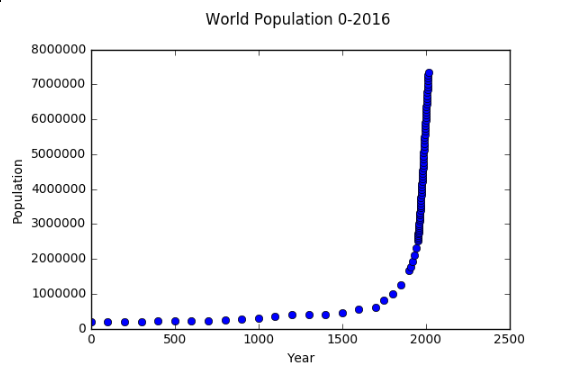
\includegraphics[width=0.7\textwidth]{worldPop}
\end{minipage}\hfill




Human population growth is decidedly exponential on a planet wide scale from the year 0 until the present day\cite{un}\cite{hyde}\cite{braben}. However, the current population growth is a product of a technology explosion beginning with the industrial revolution and further facilitated by subsequent technology advances\cite{cc}. It is unclear as to how future population growth will play out, but according to the United Nations Population Division, the most likely scenario is a slowing of population growth due to falling fertility rates worldwide, the graph from the UN World Population Prospects 2015 report\cite{un} illustrates this projected slowing.


\begin{minipage}{\textwidth}
		\centering
		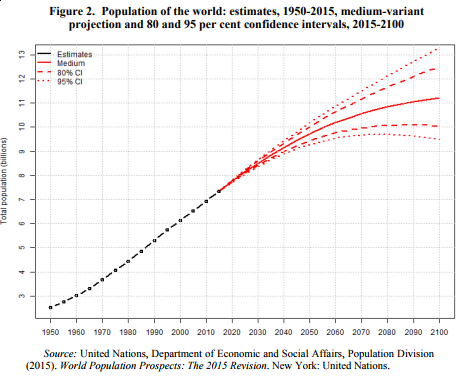
\includegraphics[width=0.7\textwidth]{unPredPop}
\end{minipage}\hfill


This data forecast suggests that the current exponential growth rate may be approaching an asymptotic limit as defined by the resources of Earth and the level of technology achieved.


In addition to this, the population of a Mars colony will be definitively limited by the artificial habitats constructed on Mars\cite{nasa}\cite{spacex} as well as the ability of the colony to produce the needed resources for survival and also population growth. As such, both the habitable space on Mars and the availability of resources will be directly tied to the level of technology. These limitations, in conjunction with the projections by the UN above suggest that a logistic growth model will provide a better base model for modeling the population of a Mars Colony.


\begin{equation} \frac{dP}{dt} = \alpha P(1-\frac{P}{K}) \end{equation}


\begin{minipage}{\textwidth}
		\centering
		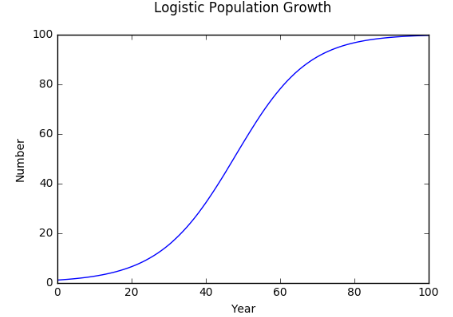
\includegraphics[width=0.6\textwidth]{logistic}
\end{minipage}\hfill




The logistic model provides a much better suited model for a population limited by some carrying capacity K than an unbounded exponential model. Indeed, combining the U.N. future population growth prediction\cite{un} with the known population data results in a graph that is well suited to be modeled with a logistic population growth model.


\begin{minipage}{\textwidth}
		\centering
		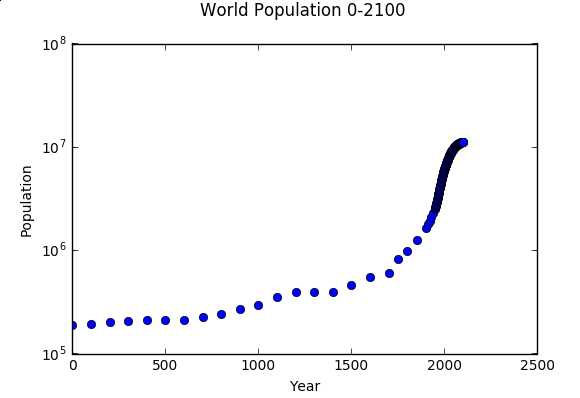
\includegraphics[width=0.7\textwidth]{futureWorldPop}
\end{minipage}\hfill




From here, another characteristic of a Mars colony needs to be factored in. A Martian colony will be more analogous to a country than the world, the reasons for this are the likelihood of a  single government, constrained resources, and that the population will likely be highly homogenous. Given this assumption, it is prudent to choose a country with the following features to base the Martian Colony model on: 
\begin{itemize}  
\item Geographically isolated
\item Scare resources
\item High technology adoption and dependence rate
\item Highly homogenous population
\end{itemize}


Given these factors, the country of Japan presents itself as the best candidate. Plotting the population of Japan\cite{japan} over time yields the following: 


\begin{minipage}{\textwidth}
		\centering
		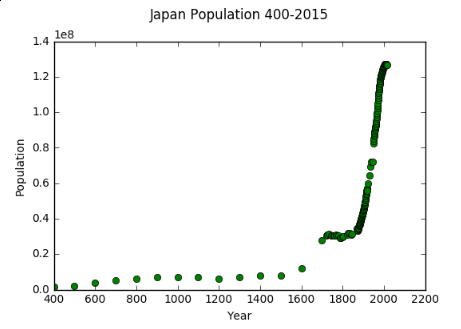
\includegraphics[width=0.7\textwidth]{japan}
\end{minipage}\hfill




Interestingly, this data\cite{japan} displays two distinct logistic growth phases, the first from 400-1800, and the second from 1800 to present day. In their paper \textit{Carrying Capacity: A Model with Logistically Varying Limits} Perrin Meyer and Jesse Ausubel present a variation on the logistic model in which the carrying capacity is not a constant, but rather a function itself\cite{cc}. 


\begin{equation} \frac{dP}{dt} = \alpha P(1-\frac{P}{K(t)}) \end{equation}


As their work demonstrates, using a second logistic function for the dynamic carrying capacity provides a model that is well fit to the population growth data of Japan. In addition, the carrying capacity should start at some nonzero value, K\textsubscript{1}  and grow logistically to a K\textsubscript{max} from there. Therefore, the equation for the logistic model of the carrying capacity is: 


\begin{equation} \frac{dK}{dt} = \alpha_{K}(K(t)-K_{1})(1-\frac{K(t)-K_{1}}{K_{max}}) \end{equation}


An analytical solution of this, as shown by Meyer \& Ausubel\cite{cc} results in:
\begin{equation} K(t) = K_{1}+ \frac{K_{max}}{1+\exp(-r_{k}(t-t_{m}))}
\end{equation}
 
 This equation takes the following shape:
 
\begin{minipage}{\textwidth}
		\centering
		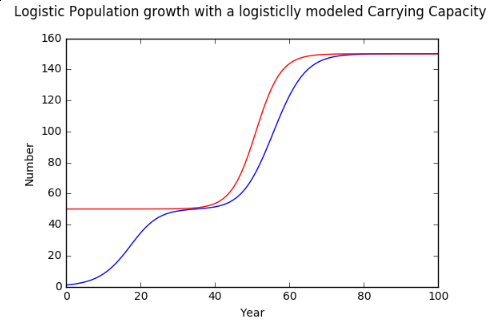
\includegraphics[width=0.7\textwidth]{logKLog}
\end{minipage}\hfill


 
 \section{Refining the Model}
 
Now that a base model has been chosen, it can be fit to the data and then conclusions as to the potential population model of a Mars colony can be extrapolated.


Focusing in on the Japan population data between 1200 and 2015 allows the leading data point to be dropped as they have little effect on the model. A first pass trial and error fit of the model to the data yields:
 
\begin{minipage}{\textwidth}
		\centering
		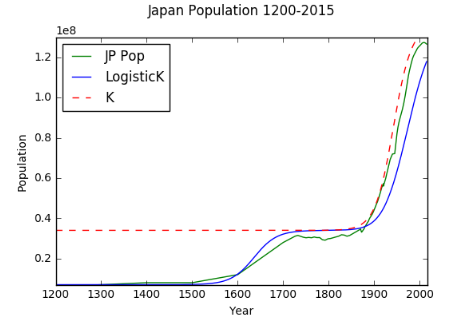
\includegraphics[width=0.7\textwidth]{firstPass}
\end{minipage}\hfill


  
  In order to assess the fit, the least squares method can be applied. However, the data set for the population of Japan\cite{un} \cite{japan} does not contain data points for each year. Therefore, the data was interpolated using the cubic spline method. Each portion of the data was interpolated individually as the periods have different data point intervals. The splines produced are below.
  
\begin{figure}[h]
	\centering
	\begin{minipage}{0.33\textwidth}
		\centering
		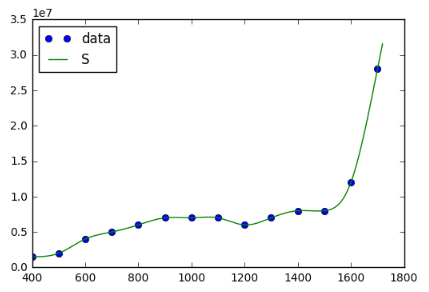
\includegraphics[width=0.9\textwidth]{spline1} % first figure itself
		\caption{first figure}
	\end{minipage}\hfill
	\begin{minipage}{0.33\textwidth}
		\centering
		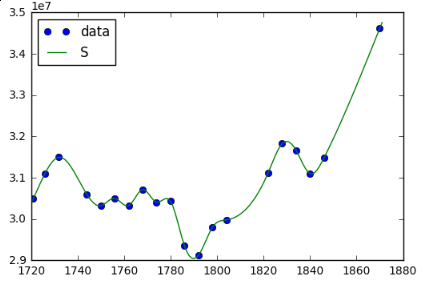
\includegraphics[width=0.9\textwidth]{spline2} % second figure itself
		\caption{second figure}
	\end{minipage}
	\begin{minipage}{0.33\textwidth}
		\centering
		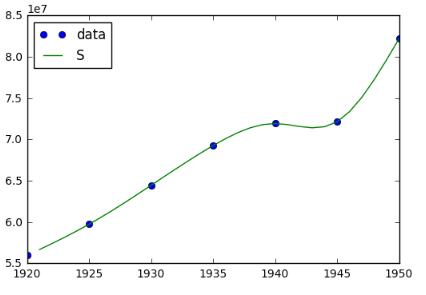
\includegraphics[width=0.9\textwidth]{spline3} % second figure itself
		\caption{second figure}
	\end{minipage}
\end{figure}


Once the data has been interpolated to produce evenly spaced a data point for each year via cubic splines, a method of nonlinear least squares fit measure can be taken to determine the fit of the model to the data, for the purpose of this model, the vertical least squares fitting method is used to find the sum of the squares of the vertical deviations, \textit{R\textsuperscript{2}} from the set of \textit{n} data points.


\begin{equation} R^2 = \frac{\Sigma(y_{fit} - y_{mean})^2} {\Sigma(y_{i} - y_{mean})^2}  \end{equation}


The \textit{R\textsuperscript{2}} for our initial guess at the model gives a fairly good fit of
\begin{equation} R^2 = 0.944 \end{equation}


In order to further refine the model, a Monte Carlo technique known as Simulated Annealing was applied for each parameter of the model,
\textit{r,r\textsubscript{K},t\textsubscript{m}}. Where \textit{r} is a constant of growth for the population, \textit{r\textsubscript{K}} is a constant of growth for the carrying capacity, and \textit{t\textsubscript{m}} determines where the inflection point of the carrying capacity logistic is placed, for ease of use in computations, \textit{t} is divided by \textit{t\textsubscript{m}} to place the inflection point in the code. The general process of Simulated Annealing is
\begin{enumerate}


\item{Start with an initial guess, \textit{S\textsubscript{0}}}
\item{Randomly generate a new guess/neighbor \textit{S\textsuperscript{'}}} based on \textit{S\textsubscript{0}}
\item{Probabilistically accept \textit{S\textsuperscript{'}} as \textit{S\textsubscript{0}} based on its fitness and the temperature of the system.}
\begin{itemize}
	\item{With a probability correlated to the temperature, take \textit{S\textsuperscript{'}} as \textit{S\textsubscript{0}} regardless of whether or not it is a better fit}
	\item{As temperature approaches 0, it becomes less and less probable that an \textit{S\textsuperscript{'}} will be accepted if it is not a better fit than \textit{S\textsubscript{0}}}
\end{itemize}
\end{enumerate}
Applying this process for 1000 iterations on each of the three parameters with a starting with 
\begin{equation} 
r=0.05,r\textsubscript{K}=0.05,t\textsubscript{m}=1.2
\end{equation}
results in


 \begin{minipage}{\textwidth}
		\centering
		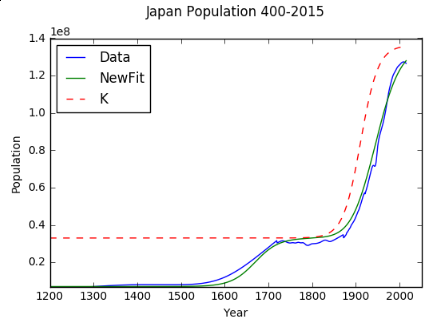
\includegraphics[width=0.7\textwidth]{japanFit}
\end{minipage}\hfill
\begin{equation} 
r=0.037,r\textsubscript{K}=0.05,t\textsubscript{m}=1.48
\end{equation}


\begin{equation} R^2 = 0.992 \end{equation}


\section{Applying the Model to Mars}


Once the model has been constructed, it can be utilized to project what the population growth of a Martian colony may look like. A significant positive of this model and the methods used to construct it is that it is trivial to refine the model further as new data is gathered as the simulated annealing process can be run continuously as new data becomes available. For now though, the usefulness of the model is limited to it's ability to be adjusted to different sets of assumptions and time frames and interpreted.


Projecting a Mars Colony population over 1000 years with the model produces: 


\begin{minipage}{\textwidth}
		\centering
		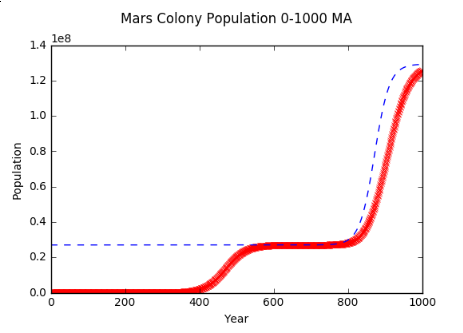
\includegraphics[width=0.7\textwidth]{mars1}
\end{minipage}\hfill


From above, it can be expected that the first 400 years of a Martian colony will be characterized by a stable, low population likely to be made up of early pioneers, scientists, and researchers. As the colony ages and humans become more proficient at living on Mars, the model predicts a population growth over about 150 years from the initial low population in the thousands up to about 25,000,000. This population growth will be facilitated by the technology advances such as indoor farming, reliable habitat modules, solar power generation, oxygen generator, and the overall improvement in the quality of life on Mars. 


This initial growth will be limited in it's growth as it approaches  25,000,000 due to the limitation of technology and overall space to live on Mars while living space is confined to artificial habitats. However, this carrying capacity imposed by technological constraints is likely to driven upwards rapidly after about 800 years of human habitation of Mars. The reason for such growth will be driven by the advent of technologies to terraform Mars into a habitable planet\cite{terraform}, thus greatly increasing the living space, and carrying capacity of a Martian colony. 

\section{Code \& Presentation}
The code developed for use in this project along with a presentation in Jupyter Notebook slides can be found at 
\begin{itemize}
\item{Code: \href{https://github.com/rugggg/MarsModel}{https://github.com/rugggg/MarsModel}}
\item{Presentation: \href{https://rugggg.github.io/MarsModel}{https://rugggg.github.io/MarsModel}}
\end{itemize}


\begin{thebibliography}{9}
\bibitem{cc} 
Perrin S. Meyer and Jesse H. Ausubel 
\textit{Technological Forecasting and Social Change 61(3):209–214, 1999. Carrying Capacity: A Model with Logistically Varying Limits }. 
 1999.
 
\bibitem{spacex} 
Elon Musk. 
\textit{Making Humans a Multiplanetary Species}.
\\\texttt{http://www.spacex.com/mars}
SpaceX, 2016.


\bibitem{nasa} 
National Aeronautics and Space Administration. 
\textit{Journey to Mars}.
\\\texttt{https://www.nasa.gov/content/journey-to-mars-overview}
NASA, 2016.


\bibitem{un} 
United Nations Department of Economic and Social Affairs, Population Division
\textit{World Population Prospects: The 2015 Revision}.
\\\texttt{https://esa.un.org/unpd/wpp/Graphs/Probabilistic/POP/TOT/}
United Nations, New York, 2015.


\bibitem{braben} 
Jean-Noël Biraben
\textit{The History of the Human Population From the First Beginnings to the Present}.
 Academic Press, San Diego, 1999.


\bibitem{japan} 
Jean-Noël Biraben
\textit{Le Point sur l'Histoire de la Population du Japon}.
1993.


\bibitem{moore} 
Moore, Gordon E.
\textit{Cramming more components onto integrated circuits}.
Intel, 1965


\bibitem{hyde} 
K. Klein Goldewijk and G. van Drecht
\textit{HYDE 3.1: Current and historical population and land cover}.
Netherlands Environmental Assessment Agency (MNP), Bilthoven, The Netherlands.


\bibitem{terraform} 
Robert M. Zubrin, Christopher P. McKay
\textit{Technological Requirements for Terraforming Mars}.
Pioneer Astronautics, NASA Ames Research Center , 1993.


\bibitem{mars} 
Clifford, S. M. and T. J. Parker
\textit{The Evolution of the Martian Hydrosphere: Implications for the Fate of a Primordial Ocean and the Current State of the Northern Plains}.
Icarus, 2001
\end{thebibliography}


\end{document}






